\chapter{Implementacja}

Rozdział ten opisuje zasadę działania programu. Program składa się z kilku kroków. Na początku użytkownik wybiera choroby, na które choruje pacjent. Następnie program wyświetla graficzną reprezentację wytycznych w formie grafu oraz wyświetla listy pól wyboru, które pozwalają na udzielanie odpowiedzi na pytania zawarte w wytycznych. Po udzieleniu odpowiedzi na pytania i kliknięciu przycisku „Dalej” program rozwiązuje problem CLP, w wyniku którego uzyskujemy listę konfliktów, które wystąpiły między wytycznymi oraz grafy wynikowe z wprowadzonymi zmianami pozwalającymi uniknąć konfliktu. Po uzyskaniu rozwiązania problemu można wybrać inne odpowiedzi na pytania i po kliknięciu przycisku „Dalej” wygenerować nowe rozwiązania problemu. Można także wybrać inne choroby za pomocą przycisku „Wybierz choroby”.

W tym rozdziale wykorzystywane są pojęcia „terapia” oraz „element terapii”. Terapia jest to pojedyncza ścieżka w grafie. Element terapii natomiast to identyfikator węzła w przypadku węzłów akcji, natomiast dla węzłów decyzji elementem terapii są identyfikator węzła i etykieta wybranej krawędzi oddzielone znakiem zapytania. Węzłami akcji są węzły, które zawierają informację o leku, jaki należy zażyć lub zabiegu, jaki należy przeprowadzić. Węzły decyzji są to z kolei węzły, które posiadają pytanie. 

W grafach może zajść sytuacja, w której należy poruszać się po ścieżkach równoległych. Sytuacja taka występuje na rysunku \ref{fig:sciezki_rownolegle}. Węzeł rozpoczynający ścieżki równoległe charakteryzuje się tym, że posiada więcej niż jedną krawędź wyjściową oraz nie ma etykiety. Natomiast węzeł kończący ścieżki równoległe posiada więcej niż jedną krawędź wejściową, nie ma etykiety oraz liczba jego krawędzi wyjściowych jest większa od zera.
\begin{figure}[H]
\centering
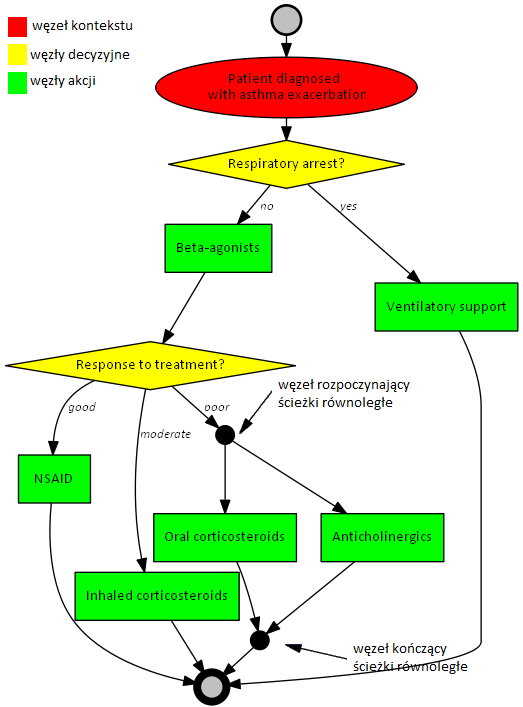
\includegraphics[width=0.7\textwidth]{img/asthma_sciezki_rownolegle.png}
\caption{Przykład ścieżek równoległych}
\label{fig:sciezki_rownolegle}
\end{figure}

Program posiada trzy istotne katalogi, które przechowują różnego typy danych. Należą do nich:
\begin{itemize}
\item{Algorytmy – zawiera pliki o rozszerzeniu dot opisujące grafy procedur medycznych chorób}
\item{Konflikty – zawiera opisy konfliktów, jakie występują między chorobami oraz zmiany, które należy wprowadzić w przypadku wystąpienia konfliktów}
\item{Grafy – zawiera zmodyfikowane grafy chorób przedstawiające aktualnie przebytą ścieżkę oraz grafy wynikowe prezentujące rozwiązania. Grafy są w dwóch formatach – tekstowym w formacie dot oraz graficznym w formacie png. Podczas zamykania programu zawartość tego katalogu jest kasowana}
\end{itemize}

Program posiada następujące klasy:
\begin{itemize}
\item{AddToTherapy - dodawanie identyfikatorów węzłów do listy opisującej konkretną terapię}
\item{ChocoClass - rozwiązanie problemu CLP}
\item{Color - kolorowanie wierzchołków i krawędzi grafów}
\item{CreateTherapies - generowanie terapii}
\item{ExecuteInteractions - wprowadzanie zmian w terapiach w przypadku wykrycia konfliktów}
\item{GoForward - przechodzenie do kolejnego węzła decyzyjnego}
\item{GraphFunctions - przydatne metody związane z grafami, np. znalezienie węzłów docelowych określonego węzła}
\item{ImageGraph - wyświetlanie grafów}
\item{MainClass - obsługa zdarzenia kliknięcia przycisku Dalej}
\item{RadioButtonList - tworzenie i obsługa zdarzeń list pól wyboru służących do udzielania odpowiedzi na pytania}
\item{Results - wyświetlanie wyników}
\item{Window - okno programu}
\end{itemize}

\section{Wybór chorób}
Celem tego kroku jest wybór tych wytycznych, które będą brane pod uwagę przy ustalaniu terapii. W katalogu Algorytmy program szuka plików posiadających rozszerzenie dot. Dla każdego takiego pliku tworzone jest pole wyboru. Pole wyboru posiada etykietę równą nazwie choroby. Utworzone pole wyboru jest następnie dodawane do globalnej listy pól wyboru o nazwie \texttt{checkBoxGroup} oraz do panelu 
znajdującego się w lewym górnym rogu okna programu (rys. \ref{fig:wybor_chorob}). 
\begin{figure}[H]
\centering
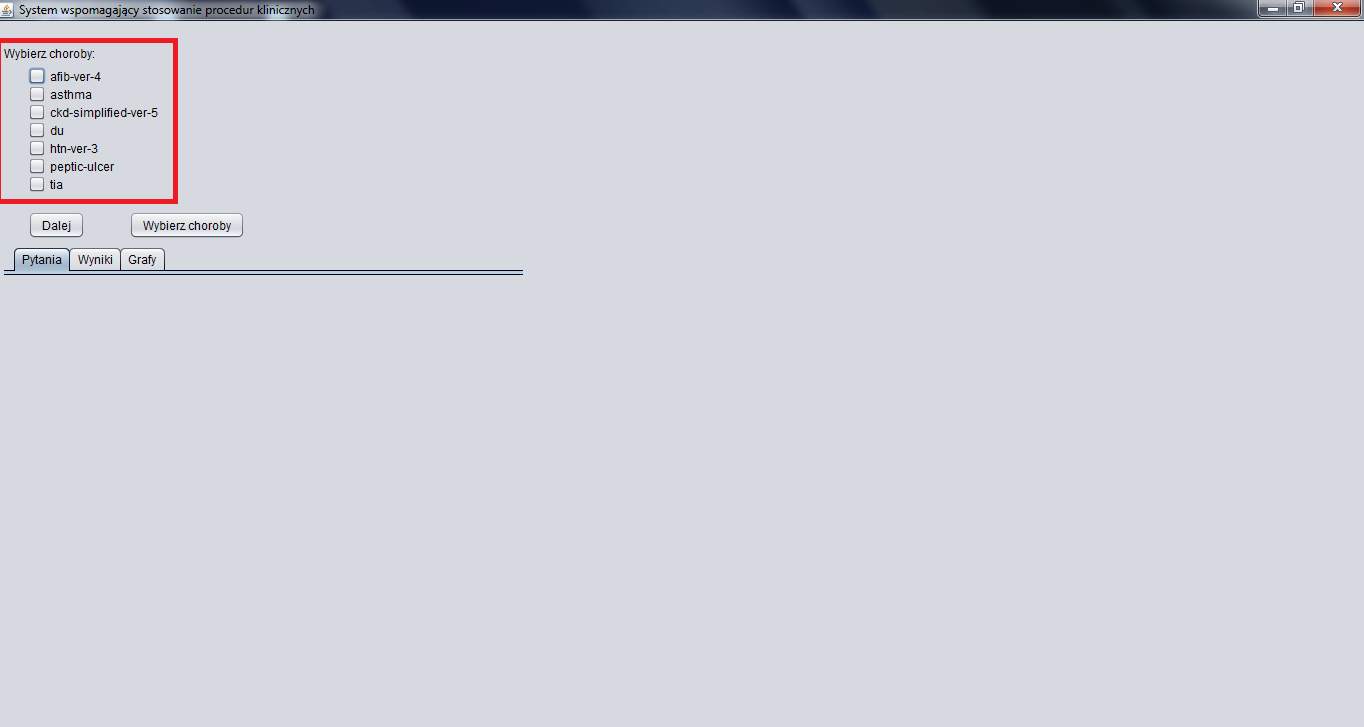
\includegraphics[width=\textwidth]{img/wybor_chorob.png}
\caption{Panel wyboru chorób}
\label{fig:wybor_chorob}
\end{figure}
Po wybraniu chorób, tzn. po kliknięciu w odpowiednie pola wyboru i kliknięciu przycisku „Dalej”, nazwy wybranych chorób są dodawane do listy o nazwie \texttt{selectedDiseases} i program przechodzi do fazy wyświetlania grafów oraz udzielania odpowiedzi na pytania. 

\section{Wyświetlanie grafów oraz udzielanie odpowiedzi na pytania}
Ten krok pozwala na utworzenie graficznej reprezentacji wytycznych oraz wybór ścieżki grafu zgodnej z danymi pacjenta. Po wybraniu chorób i kliknięciu przycisku „Dalej” program dla każdej choroby odczytuje za pomocą metody \texttt{GraphFunctions.getGraph} grafy z pliku o rozszerzeniu dot. Następnie, program pobiera korzenie każdego z grafów za pomocą metody \texttt{GraphFunctions.get\-StartNode}. W następnym etapie program wywołuje metodę \texttt{GoForward.goForward}, która przemieszcza się po grafie do momentu, gdy napotka pierwszy węzeł decyzji. Parametrem metody \texttt{goForward} jest m.in. korzeń grafu.

Najpierw \texttt{goForward} dodaje aktualny węzeł do listy elementów terapii. Następnie program wykonuje pętlę while, której warunek kontynuacji obejmuje trzy przypadki. Pętla ta stanowi część metody \texttt{goForward}. Pierwszy warunek sprawdza, czy węzeł posiada jedną krawędź wyjściową. Drugi warunek sprawdza, czy węzeł rozpoczyna ścieżki równoległe, a trzeci czy węzeł kończy ścieżki równoległe. 

Pierwszy warunek jest sprawdzany w kolejnej pętli while, aby dodać do listy elementów terapii wszystkie węzły, które mają tylko jedną krawędź wyjściową, czyli droga, po której należy się poruszać jest jednoznacznie określona. 
Po wykonaniu tej pętli while uzyskujemy węzeł, który jest liściem (nie posiada żadnej krawędzi wyjściowej), albo ma więcej niż jedną krawędź wyjściową.

W kolejnym kroku sprawdzany jest dla aktualnego węzła drugi warunek w instrukcji if, czyli czy węzeł rozpoczyna ścieżki równoległe. Jeśli jest on spełniony, wywoływana jest metoda \texttt{parallel\-Path}. Metoda ta jest wywoływana również w dla trzeciego przypadku, czyli gdy uzyskany węzeł kończy ścieżki równoległe, a program nie przeszedł jeszcze przez wszystkie te ścieżki. Metoda \texttt{parallel\-Path} jest w postaci pętli while, która działa dopóki program nie przejdzie przez wszystkie ścieżki równoległe związane z węzłem rozpoczynającym ścieżki równoległe i uzyskany węzeł nie jest węzłem zawierającym pytanie. Pętla while zapisuje do listy elementów terapii wszystkie przebyte po drodze węzły.  

Po wywołaniu metody \texttt{goForward} program wywołuje metodę \texttt{Color.color}, która zaznacza przebytą ścieżkę w grafie. Metoda \texttt{goForward} do listy list o nazwie \texttt{dataIdList} dodawała identyfikatory węzłów, na które program natrafił. Dzięki \texttt{dataIdList} metoda \texttt{color} może pokolorować kontury przebytych węzłów oraz przebyte krawędzie, a także je pogrubić. 
 
Po wywołaniu metody \texttt{color} wywołana zostaje metoda \texttt{ImageGraph.newImageGraph}, której zadaniem jest wygenerowanie i wyświetlenie nowego obrazu grafu. Na początku metoda zapisuje do pliku wynik metody \texttt{toString} wywołanej dla grafu. Następnie wywoływana jest metoda \texttt{ImageGraph.getImageGraphPath}, która uruchamia program dot.exe i tworzy z zapisanego wcześniej pliku tekstowego graf w postaci obrazu w formacie PNG. W kolejnym kroku metoda \texttt{ImageGraph.newImageGraph} tworzy obiekt klasy \texttt{BufferedImage} z wygenerowanym w poprzednim kroku obrazem. Później metoda dokonuje skalowania obrazu tak, aby mógł on się zmieścić na etykiecie. 

Jeśli szerokość lub wysokość obrazu przekracza próg 900 pikseli, obraz zmniejszany jest do 2/3 wielkości tak, aby był on czytelny (w tym przypadku do etykiety dodawane są suwaki). Ponadto, jeżeli szerokość i wysokość obrazu jest mniejsza od wielkości etykiety, to na etykiecie umieszczany jest obraz bez skalowania, w skali 1:1.
 
Ostatnim krokiem jest wywołanie metody \texttt{RadioButtonList.createRadioButtonList}. Metoda ta dla każdego elementu terapii, który posiada znak zapytania tworzy panel. Elementy terapii zwierające znak zapytania odpowiadają krokom decyzyjnym. Pierwszym elementem panelu jest etykieta węzła. Pozostałe elementy stanowią pola wyboru z etykietami, których wartości są równe etykietom krawędzi węzła decyzyjnego. Do tych pól wyboru dodawany jest jeszcze jeden z etykietą „brak wartości”, przydatny w sytuacji, gdy nie znamy jeszcze danych. Część elementu terapii po znaku zapytania pozwala na przechowanie informacji o wyborze aktywnego pola wyboru. Na końcu tworzony jest jeszcze jeden panel, tym razem dla pytania, na które jeszcze nie została udzielona odpowiedź, dla niego zaznaczone jest pole wyboru z etykietą „brak wartości”. Przy pierwszym wyświetleniu grafu tworzony jest tylko ten panel. Ponadto, dla każdego pola wyboru przypisywane jest zdarzenie \texttt{RadioButtonList.updateRadioButtonList}.

Metoda \texttt{updateRadioButtonList} na początku szuka elementu w liście elementów terapii, którego dotyczy pytanie. Jeśli zaznaczone pole wyboru ma etykietę „brak wartości”, usuwane są wszystkie elementy terapii od elementu, którego dotyczy pytanie, do ostatniego elementu listy. W sytuacji tej cofamy się z udzielaniem odpowiedzi na pytania do jednego z poprzednich pytań.

Jeśli natomiast zaznaczone pole wyboru nie posiada etykiety równej „brak wartości” i nie istnieje element na liście elementów terapii, który jest związany z pytaniem, to do tej listy dodawany jest element o wartości równej \texttt{question?answer}, gdzie \texttt{answer} jest parametrem metody \texttt{updateRadioButtonList} o wartości równej etykiecie krawędzi, z którą jest związane zaznaczone pole wyboru. W sytuacji tej użytkownik udziela po raz pierwszy odpowiedzi na pytanie. 

Jeśli istnieje element związany z pytaniem, to w liście elementów terapii podmieniany jest element, który jest związany z pytaniem na wartość \texttt{question?answer}, a następnie usuwane są wszystkie elementy listy terapii, które się znajdują za podmienionym elementem. 

Następnie pod węzeł o nazwie next podstawiany jest węzeł, który jest pierwszym węzłem krawędzi o etykiecie \texttt{answer} wychodzącej z węzła o identyfikatorze \texttt{question}. W kolejnym kroku wywoływana jest metoda \texttt{goForward}, która jako parametr przyjmuje m.in. węzeł \texttt{next}. 

Metoda \texttt{updateRadioButtonList} w kolejnym kroku odznacza wszystkie węzły i krawędzie i następnie koloruje je na nowo na podstawie listy elementów terapii. Tworzony jest także nowy obraz grafu za pomocą metody \texttt{newImageGraph}. Na końcu tworzona jest nowa lista pytań i odpowiedzi za pomocą metody \texttt{createRadioButtonList}. 


Ostatecznie grafy prezentowane są po prawej stronie ekranu na zakładkach. Każda zakładka dotyczy wytycznych związanych z jedną z wybranych chorób. Z lewej strony ekranu pojawiają się natomiast zakładki z listami pól wyboru. W tym przypadku również jedna zakładka dotyczy jednej choroby. Listy pól wyboru pozwalają na udzielanie odpowiedzi na pytania zawarte w wytycznych klinicznych. Przykład wyświetlanych grafów przedstawiono na rys. \ref{fig:wyswietlanie_grafow}.
\begin{figure}[H]
\centering
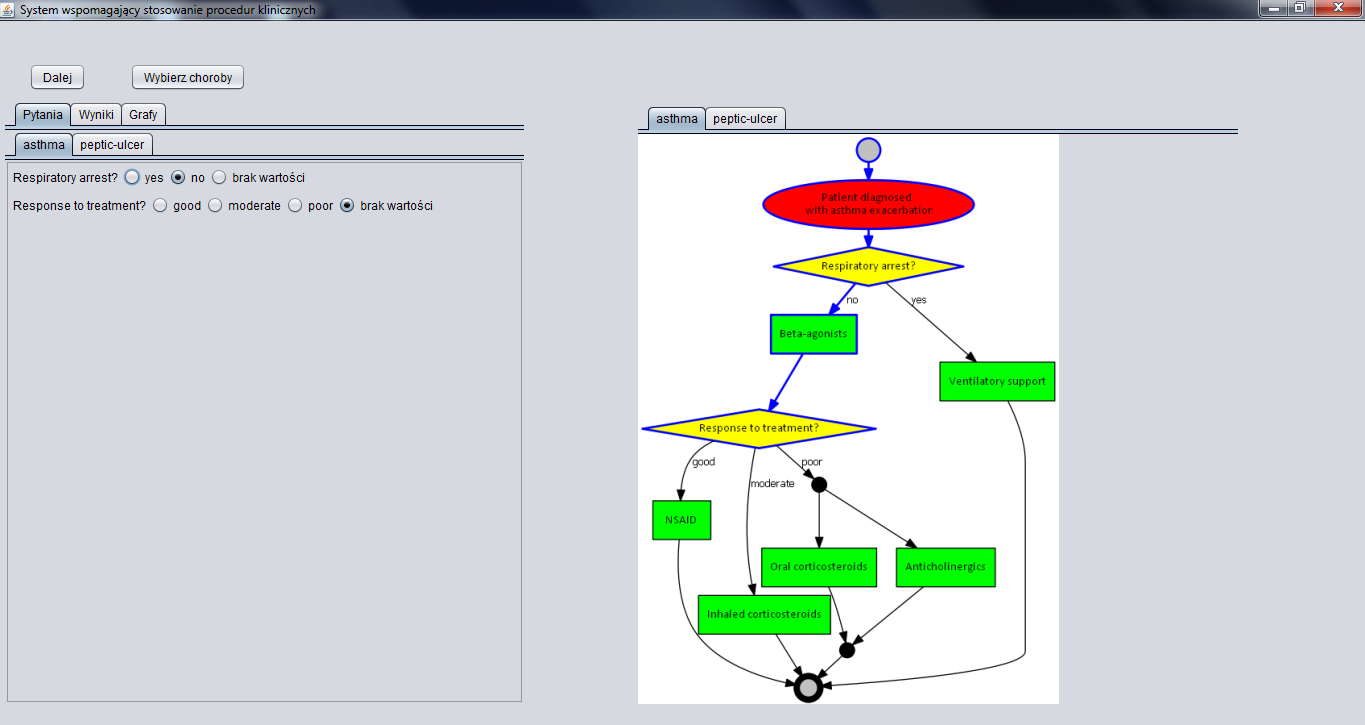
\includegraphics[width=\textwidth]{img/wyswietlanie_grafow.png}
\caption{Wyświetlanie grafów}
\label{fig:wyswietlanie_grafow}
\end{figure}

\section{Wyszukiwanie konfliktów}
Celem tego kroku jest znalezienie konfliktów występujących między wytycznymi. Na początku program szuka w katalogu konflikty plików o rozszerzeniu txt oprócz pliku nazwy.txt. Następnie program sprawdza, czy można użyć pliku z konfliktami. Nazwa każdego pliku z konfliktami składa się z listy chorób oddzielonych przecinkami, których dotyczą konflikty. Jeśli jakaś choroba z tej listy znajduje się w wybranych podczas działania programu chorobach, plik zostaje użyty. Każdy plik z konfliktami składa się z linii złożonych z dwóch części. Pierwsza część zawiera elementy, których jednoczesne wystąpienie powoduje wystąpienie konfliktu. Elementy te są oddzielone spacją. Druga część linii zawiera zmiany, jakie należy wprowadzić w przypadku zaistnienia konfliktu. Zmiany te są oddzielone od siebie przecinkami. Jeśli plik zostaje użyty, do listy \texttt{conflictsList} dodawane są konflikty, a do listy \texttt{interactionsList} zmiany. Ponadto, do listy \texttt{additionalQuestions} dodawane są elementy opisujące konflikt, które rozpoczynają się znakiem „\&”. Dla elementów tych będzie trzeba udzielić odpowiedzi, ponieważ są to dane, które nie wystąpiły jawnie w wytycznych. Elementy konfliktów rozpoczynające się od „not” dodawane są do listy \texttt{notConflictElems}. Następnie program tworzy okienko dialogowe, które pozwala udzielić odpowiedzi na dodatkowe pytania. Pytania mogą być dwóch typów. Pierwszy typ występuje, gdy element nie posiada znaku równości, mniejszości ani większości. Wtedy udzielana odpowiedź ma postać tak/nie. Drugi typ to „zmienna operator liczba”. Operator może być postaci „=”, „>”, „<”, „>=” lub „<=”. Dla tego typu elementu podawana jest wartość liczbowa w okienku dialogowym, a program sprawdza czy podana liczba spełnia warunek występujący w elemencie. 

Po udzieleniu odpowiedzi na wszystkie dodatkowe pytania program przechodzi do kolejnej części wyszukiwania konfliktów o nazwie \texttt{solveNextPart}. Metoda \texttt{solveNextPart} najpierw wywołuje metodę \texttt{findSolutions}. Metoda ta dla każdego konfliktu wykonuje szereg operacji. Najpierw metoda sprawdza, czy konflikt znajduje się na liście \texttt{foundConflicts}. Lista \texttt{foundConflicts} zawiera konflikty, które zostały znalezione przez program. Jeśli konflikt nie znajduje się na tej liście tworzony jest obiekt klasy \texttt{Solver}. Następnie dodawane są zmienne na podstawie wcześniej udzielonych odpowiedzi na dodatkowe pytania. Dokonuje tego metoda \texttt{setAdditionalVariables}. Metoda ta sprawdza, czy pytanie jest typu tak/nie czy odpowiedzią na pytanie jest wartość liczbowa. W pierwszej sytuacji, jeśli odpowiedź jest równa tak, program tworzy zmienną biblioteki Choco typu \texttt{IntVar} o wartości równej jeden. Jeżeli odpowiedź jest równa nie, program tworzy zmienną \texttt{IntVar} o wartości równej zero. Jeśli odpowiedzią na pytanie jest wartość liczbowa, program tworzy zmienną \texttt{IntVar} o wartości równej podanej liczbie. 

Po wykonaniu metody \texttt{setAdditionalVariables} program wywołuje metodę \texttt{setVariables}. Metoda ta dla każdej choroby tworzy tablicę terapii. W kolejnym kroku dla każdej terapii choroby tworzona jest zmienna \texttt{IntVar} o nazwie „choroba\_terapiaX”, gdzie choroba jest nazwą choroby, a X jest numerem terapii. Zmienna ta przyjmuje wartości zero, gdy  określona terapia nie zostaje użyta lub jeden, gdy zostaje użyta. Zmienna jest zapisywana w tablicy terapii. Następnie program tworzy listę \texttt{notConflictElemsTherapy}, do której dodawane są te elementy konfliktu z listy \texttt{notConflictElems}, które nie znajdują się na liście elementów konkretnej terapii, ale znajdują się w grafie związanym z terapią. Elementy listy \texttt{notConflictElemsTherapy} są unikalne, nie powtarzają się. Następnie program tworzy tablicę \texttt{vars}, która będzie zawierała zmienne wchodzące w skład pojedynczej terapii. W kolejnym kroku dla każdego elementu listy \texttt{notConflictElemsTherapy} w tablicy \texttt{vars} zapisywane są zmienne o nazwie „not\_X”, gdzie X jest elementem terapii z \texttt{notConflictElemsTherapy}. Zmienna ta przyjmuje wartość 0, gdy zmienna związana z elementem terapii jest równa 1 i odwrotnie. Ponadto, dla każdego elementu terapii program zapisuje zmienną w tablicy \texttt{vars}. Jeśli zmienna posiada dawkę, tworzona jest zmienna „X\_dosage”, gdzie X jest elementem terapii. Po dodaniu wszystkich elementów określonej terapii program dodaje do \texttt{vars} zmienną dodatkową, która pozwala na skorzystanie tylko z jednej terapii dla każdej z chorób. Następnie program dodaje ograniczenie polegające na tym, że zmienna „choroba\_terapiaX” przyjmuje wartość jeden, gdy suma zmiennych należących do tablicy \texttt{vars} jest równa wielkości tej tablicy. Wartość zero przyjmuje zmienna terapii w przeciwnym razie. Po przejściu przez wszystkie terapie określonej choroby program dodaje ograniczenie polegające na tym, że suma zmiennych terapii choroby ma być równa jeden, czyli dla każdej choroby ma zostać użyta tylko jedna terapia. 

Po wykonaniu metody \texttt{setVariables} program dodaje ograniczenia konfliktów. Najpierw dodawane są ograniczenia tych konfliktów, które występowały w poprzednich iteracjach pętli for i po których dodaniu zostało wygenerowane poprawne rozwiązanie (są to konflikty, które znajdują się na liście \texttt{avoidedConflicts}). Następnie dodawane jest ograniczenie konfliktu, które odpowiada aktualnej iteracji pętli. Metoda dodawania ograniczeń konfliktu ma nazwę \texttt{setConflictConstraint}. Metoda ta najpierw tworzy listę o nazwie \texttt{constraintsList}. Następnie metoda wywołuje pętlę for dla każdego elementu wchodzącego w skład konfliktu. Pętla ta najpierw sprawdza czy element konfliktu zawiera znak równości, mniejszości lub większości. Jeśli tak nie jest, ale element konfliktu rozpoczyna się od operatora „not”, program dodaje ograniczenie „not(zmienna=1)” do listy \texttt{constraintsList}. Jeśli element konfliktu nie zawiera znaku równości, mniejszości ani większości i nie rozpoczyna się od „not”, program dodaje ograniczenie postaci „zmienna=1” do listy \texttt{constraintsList}. Jeżeli natomiast element konfliktu zawiera znak równości, mniejszości lub większości, metoda wywołuje metodę o nazwie \texttt{conflictWithDosage}. Metoda ta dodaje ograniczenie postaci „zmienna operator wartość” do listy \texttt{constraintsList} w przypadku, gdy nazwa zmiennej rozpoczyna się od „\&”, czyli jest to zmienna dodatkowa, na którą udzieliło się odpowiedzi w okienku dialogowym. Jeśli zmienna nie rozpoczyna się od „\&”, dodawane są dwa ograniczenia do \texttt{constraintsList}. Pierwsze ograniczenie jest postaci „zmienna=1”, drugie natomiast jest postaci „zmienna\_dosage operator wartość”. Oba te ograniczenia są dodawane do listy \texttt{constraintsList}. Po wykonaniu pętli dla każdego elementu konfliktu metoda tworzy z listy \texttt{constraintsList} tablicę, a następnie dodaje do solvera ograniczenie postaci not(and(ograniczenia)). 

W następnym kroku program wywołuje metodę \texttt{findSolution} obiektu klasy \texttt{Solver}, które dokonuje znalezienie rozwiązania problemu. Jeśli rozwiązanie istnieje, do \texttt{avoidedConflicts} dodawany jest numer konfliktu na liście \texttt{conflictsList}. Jeśli natomiast nie ma rozwiązania, do \texttt{foundConflicts} dodawany jest konflikt oraz do \texttt{interactionsList} dodawane są zmiany odpowiadające konfliktowi. Ponadto, gdy nie ma rozwiązania program wywołuje metodę \texttt{execute\-Interactions}, która dokonuje zmian w terapiach, a także program wywołuje rekurencyjnie metodę \texttt{findSolutions}, aby sprawdzić, czy wprowadzone zmiany nie spowodowały wystąpienia konfliktów, dla których już dokonało się przeglądu, oraz aby sprawdzić kolejne konflikty. Po wywołaniu metody \texttt{findSolutions} program ustawia wartość stop na true, co powoduje, że program nie sprawdza wystąpienia kolejnych konfliktów, ponieważ zrobiła już to wywołana rekurencyjnie metoda \texttt{findSolutions}. 

Ostatecznie, program dokonuje rozwiązania problemu z tymi ograniczeniami w postaci konfliktów, które znajdują się na liście \texttt{avoidedConflicts}. Po wygenerowaniu pierwszego rozwiązania program tworzy listę o nazwie \texttt{solutions}. Następnie w pętli do/while, która działa dopóki istnieje kolejne rozwiązanie, program zapisuje do zmiennej \texttt{solution} po przecinku nazwy zmiennych terapii, które posiadają wartość równą jeden. Następnie, jeśli zmienna \texttt{solution} nie znajduje się jeszcze w liście \texttt{solutions}, zmienna dodawana jest do tej listy. Na końcu program do listy \texttt{therapies} dodaje rozwiązania. Polega to na tym, że dla każdego elementu listy \texttt{solutions} o nazwie \texttt{elem} program tworzy listę o nazwie \texttt{therapiesSolution}. Następnie tworzy tablicę o nazwie \texttt{array} zawierającą elementy, które były w zmiennej \texttt{elem} rozdzielone przecinkami. W kolejnym kroku dla każdej choroby znajdującej się w liście \texttt{diseases} szuka elementu w tablicy \texttt{array}, którego nazwa rozpoczyna się od nazwy choroby. Następnie do listy \texttt{therapiesSolution} dodaje listę z \texttt{therapiesDiseases} o numerze równym numerowi choroby i podnumerze równym X znajdującym się w nazwie zmiennej terapii „choroba\_terapiaX”. Lista \texttt{therapiesDiseases} zawiera terapie wszystkich wybranych chorób zgodne z udzielonymi odpowiedziami na pytania znajdujące się w wytycznych. Na końcu program wywołuje metodę \texttt{setResults}, która pozwala na zaprezentowanie wyników. 

\section{Wyświetlanie wyników}
Ostatni krok polega na wyświetleniu grafów wynikowych prezentujących rozwiązania, a także utworzeniu listy znalezionych konfliktów wraz z wprowadzanymi zmianami. Program prezentuje wyniki za pomocą metody \texttt{setResults}. Na początku metoda wywołuje inną metodę o nazwie \texttt{setGraphs}. Zajmuje się ona wyświetleniem wyników w postaci grafów. Najpierw metoda usuwa wszystkie zakładki z rozwiązaniami z zakładki „Grafy”. W kolejnym kroku wywołuje dwie pętle, z których druga się zawiera w pierwszej. Pierwsza pętla porusza się po rozwiązaniach, druga po terapiach pojedynczego rozwiązania. Dla każdej terapii, która jest związana z określoną chorobą, tworzony jest odpowiedni graf. Następnie metoda wywołuje pętlę po grupach zmian poszczególnych konfliktów oraz po pojedynczych zmianach. 

Dla każdej zmiany sprawdzany jest jej typ. Zmiany mogą być kilku typów. Pierwszy typ to „replace X with Y”, który polega na tym, że węzeł X zamienia się na węzeł Y. Kolejny typ to „add X before/after Y”, który charakteryzuje się tym, że węzeł X jest dodawany przed lub po elemencie Y w zależności od tego, czy zostało użyte before czy after. Kolejnym typem jest „remove X”, które polega na usunięciu węzła X. Istnieją jeszcze typy zmian postaci „increase\_dosage X Y”, „decrease\_dosage X Y”, które powodują zwiększenie lub zmniejszenie dawki węzła X o Y. Ostatnim typem jest „change\_dosage X Y”, które polega na zmianie dawki węzła X na wartość Y.  

Jeśli zmiana jest typu „replace”, najpierw program szuka węzła o identyfikatorze równym elementowi, który należy zamienić. Po znalezieniu takiego węzła z pliku nazwy.txt odczytywana jest etykieta elementu, który ma się znaleźć na miejscu zamienianego elementu. Etykieta jest następnie zapisywana jako etykieta znalezionego węzła. Ponadto, program zamienia identyfikator znalezionego węzła na nowy. Jeśli zmiana jest typu „add”, program szuka węzła, przed lub za którym ma zostać umieszczony nowy węzeł. Następnie program tworzy nowy węzeł, nadaje mu etykietę pobraną z pliku nazwy.txt i dodaje węzeł do grafu. Następnie, jeżeli element, względem którego ma zostać wstawiony nowy węzeł jest postaci „pytanie?odpowiedź”, dla krawędzi, która ma etykietę „odpowiedź”, program ustawia węzeł docelowy krawędzi na nowo utworzony węzeł. Następnie, program tworzy nową krawędź, której węzłem źródłowym jest nowo utworzony węzeł, a węzłem docelowym jest węzeł docelowy krawędzi o etykiecie „odpowiedź”. Powoduje to umieszczenie nowego węzła na początku krawędzi z etykietą „odpowiedź”. Jeżeli natomiast element, względem którego ma być wstawiony nowy węzeł nie jest typu „pytanie?odpowiedź”, mogą wystąpić dwa przypadki. Pierwszy przypadek występuje, gdy zmiana jest typu „add X after Y”, drugi, gdy zmiana jest typu „add X before Y”. Dla tych sytuacji nowy węzeł jest umieszczany odpowiednio za lub przed węzłem Y. 

W przypadku, gdy typ zmiany to „remove”, program przypisuje znalezionemu węzłowi atrybut style na wartość „invis”, atrybut fixedsize na „true” oraz atrybuty height i width na „0”. Powoduje to, że węzeł usunięty staje się niewidoczny na tworzonym grafie. Dla typów zmian „increase\_dosage”, „decrease\_dosage” i „change\_dosage” odpowiednio zmienia się końcową część etykiety z nawiasami kwadratowymi, która przedstawia dawkę. Na końcu metoda \texttt{setGraphs} dla każdego grafu wywołuje metodę \texttt{color} zaznaczającą przebyte węzły i krawędzie, a następnie metodę \texttt{newImageGraph}, która powoduje wygenerowanie grafu w postaci obrazkowej. 

Po wywołaniu metody \texttt{setGraphs} program tworzy rozwiązania tekstowe. Polega to na utworzeniu dla każdego rozwiązania i dla każdej choroby pojedynczego rozwiązania dwóch pól tekstowych. Pierwsze z nich przedstawia etykiety przebytych węzłów, a drugie ich identyfikatory. Etykietę węzła otrzymuje się przez znalezienie węzła o identyfikatorze równym elementowi terapii, a następnie odczytanie jego etykiety. Dla węzła pytającego program wypisuje dodatkowo etykietę wybranej krawędzi. Jeśli jest taka potrzeba, program szuka etykiety węzła w pliku nazwy.txt. Drugie pole tekstowe, z identyfikatorami, program tworzy wypisując elementy terapii z listy. Elementy są oddzielone od siebie znakiem nowej linii. Po utworzeniu pól tekstowych program umieszcza je na panelu, który jest z kolei umieszczany na zakładce. Na końcu program wypisuje w odpowiednim polu tekstowym konflikty i związane z nimi zmiany. Podczas wypisywania konfliktów i zmian program szuka odpowiednich etykiet węzłów w grafie lub w pliku nazwy.txt. 

\section{Przykładowe działanie programu}
W tym przykładzie zostały wybrane dwie choroby: migotanie przedsionków (ang. attrial fibrillation, rys. \ref{fig:afib_przyklad}) oraz przewlekła choroba nerek (ang. chronic kidney disease, rys. \ref{fig:ckd_przyklad}).
\begin{figure}[H]
\centering
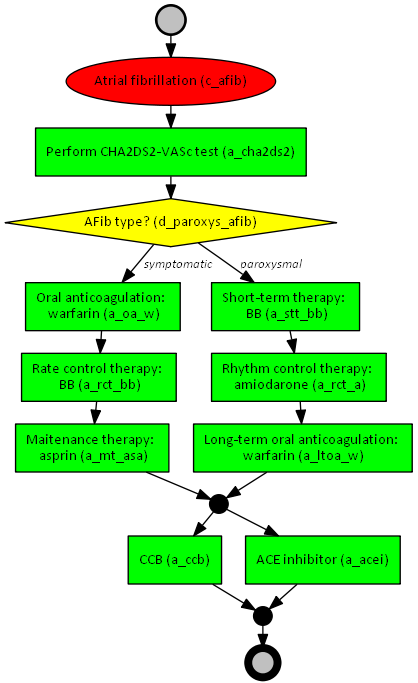
\includegraphics[scale=0.5]{img/afib-ver-4_przyklad.png}
\caption{Wytyczne dla migotania przedsionków}
\label{fig:afib_przyklad}
\end{figure}
\begin{figure}[H]
\centering
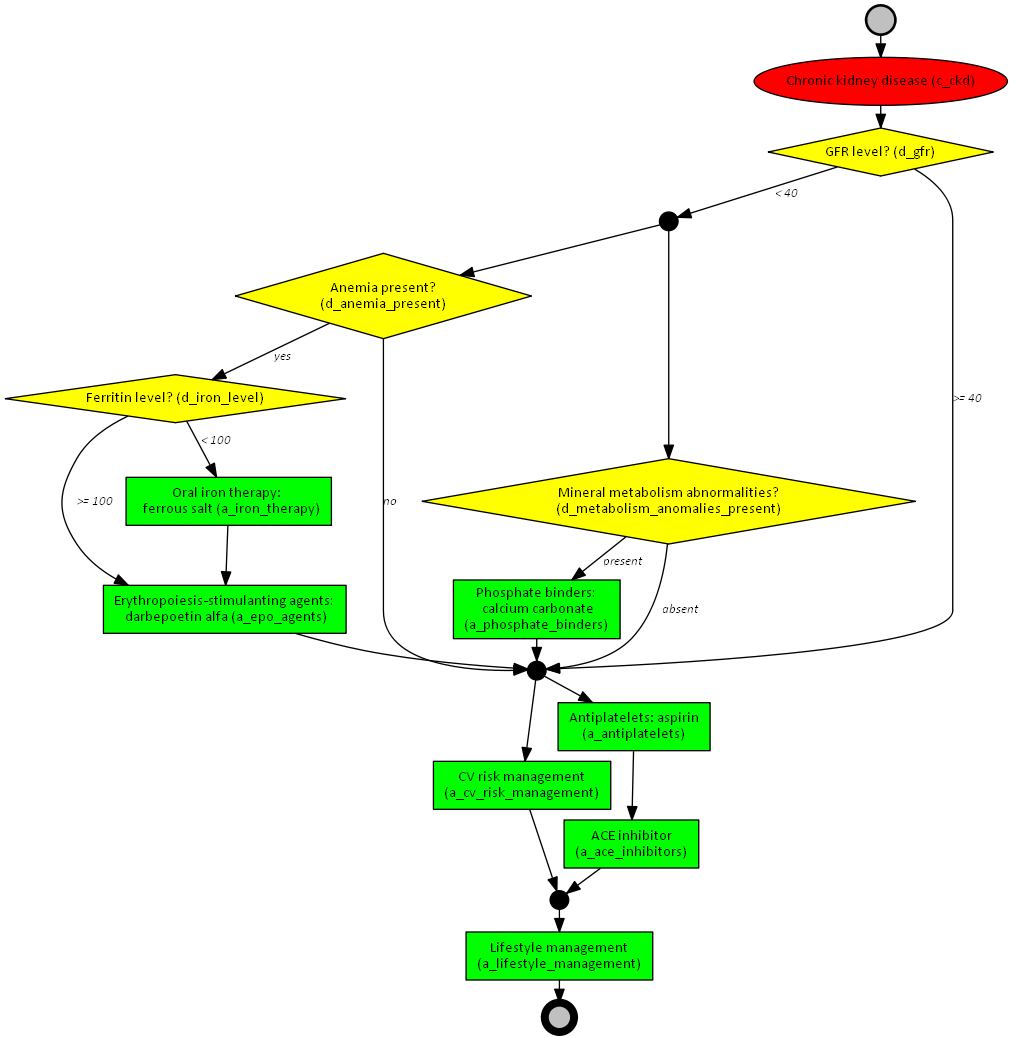
\includegraphics[scale=0.4]{img/ckd-simplified-ver-5_przyklad.png}
\caption{Wytyczne dla przewlekłej choroby nerek}
\label{fig:ckd_przyklad}
\end{figure}
Węzły grafów posiadają etykiety zawierające na końcu w nawiasach identyfikatory swoich węzłów. Dla pierwszej z chorób na początku program zatrzymuje się na pierwszym pytaniu „AFib Type?”, zapisując wcześniej do listy elementów terapii węzeł startowy, węzeł określający chorobę oraz węzeł „Perform CHA2DS2-VASc test”. Po udzieleniu odpowiedzi „paroxysmal” program dodaje do listy „d\_paroxys\_afib?paroxysmal”, a następnie trzy węzły: „Short-term therapy: BB”, „Rhythm control therapy: amiodarone” i „Long-term oral anticoagulation: warfarin”. Następnie program dodaje węzeł rozpoczynający ścieżki równoległe, następnie dwa węzły znajdujące się na ścieżkach równoległych (najpierw węzeł „CCB”, następnie węzeł „ACE inhibitor”), a później węzeł kończący ścieżki równoległe. Ostatecznie program dodaje węzeł końcowy grafu. 

Dla drugiej choroby, czyli przewlekłej choroby nerek, program zatrzymuje się na pytaniu „GFR level?”, dodając po drodze węzeł startowy oraz węzeł choroby. Po udzieleniu odpowiedzi „<40” program dodaje do listy „d\_gfr?<40”, a następnie trafia na węzeł rozpoczynający ścieżki równoległe, który również jest dodawany do listy. W kolejnym kroku program zatrzymuje się na  pytaniu znajdującym się na lewej równoległej krawędzi: „Anemia present?”. Po udzieleniu odpowiedzi „no” program dodaje do listy „d\_anemia\_present?no”, a następnie wraca do prawej krawędzi równoległej i zatrzymuje się na pytaniu „Mineral metabolism abnormalities?”. Po udzieleniu odpowiedzi „absent” program dodaje do listy „d\_metabolism\_anomalies\_present?absent”. Następnie program umieszcza na liście węzeł kończący ścieżki równoległe, który jednocześnie rozpoczyna kolejne ścieżki równoległe. W kolejnym kroku program dodaje element znajdujący się na lewej krawędzi równoległej, czyli „CV risk management”, a następnie elementy znajdujące się na prawej krawędzi równoległej, czyli „Antiplatelets: aspirin” oraz „ACE inhibitor”. Ostatecznie dodawany jest węzeł kończący ścieżki równoległe, węzeł „Lifestyle management” oraz węzeł końcowy grafu.

Po udzieleniu odpowiedzi na pytania i kliknięciu przycisku „Dalej” program przechodzi do fazy wyszukiwania konfliktów. Najpierw program odczytuje plik z konfliktami dotyczącymi migotania przedsionków oraz przewlekłej choroby nerek. Plik ten ma następującą zawartość:
\begin{verbatim}
c_htn c_ckd:remove a_step1_acei,remove a_step1_ccb
c_afib c_ckd c_htn:remove a_step3_diuretric
c_afib c_ckd:replace a_antiplatelets with warfarin,replace a_rct_a with BB
c_afib c_ckd &CHA2DS2-VASc>2:replace a_mt_asa with warfarin2
c_afib c_ckd &CHA2DS2-VASc<=1:replace a_oa_w with aspirin1,
replace a_ltoa_w with aspirin2
\end{verbatim}
Następnie program uruchamia okienko dialogowe z jedną zmienną do uzupełnienia o nazwie CHA2\-DS2-VASc. Po przypisaniu do tej zmiennej wartości 5 program zaczyna wyszukiwać konflikty. Ostatecznie program znajduje dwa konflikty: (c\_afib c\_ckd) oraz (c\_afib c\_ckd \&CHA2DS2-VASc>2). Pierwsze dwa konflikty nie wystąpiły, ponieważ nie wybrano choroby o identyfikatorze c\_htn. Ostatni konflikt nie wystąpił natomiast dlatego, że zmienna CHA2DS2-VASc przyjmuje wartość większą od 1.

W kolejnym kroku program tworzy zmodyfikowane grafy wynikowe, które zawierają zmiany wprowadzone w celu uniknięcia konfliktów. Graf dla migotania przedsionków został przedstawiony na rys. \ref{fig:afib_rozw}, natomiast graf dla przewlekłej choroby nerek jest na rys. \ref{fig:ckd_rozw}. W grafie dla migotania przedsionków zamieniony został węzeł „Maintenance therapy: aspirin” na węzeł „Maintenance therapy: Warfarin” oraz węzeł „Rhytm control therapy: amiodarone” na węzeł „BB”. W grafie dla przewlekłej choroby nerek został zamieniony węzeł „Antiplatelets: aspirin” na węzeł „Warfarin”.
\begin{figure}[H]
\centering
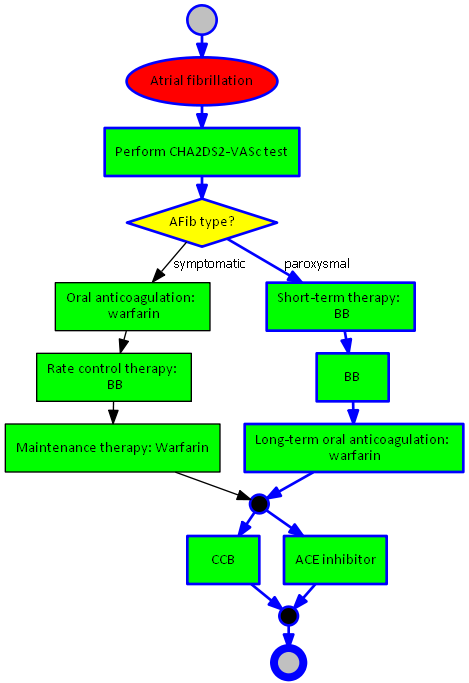
\includegraphics[scale=0.5]{img/rozwiazanie1afib-ver-4_przyklad.png}
\caption{Wytyczne dla migotania przedsionków}
\label{fig:afib_rozw}
\end{figure}
\begin{figure}[H]
\centering
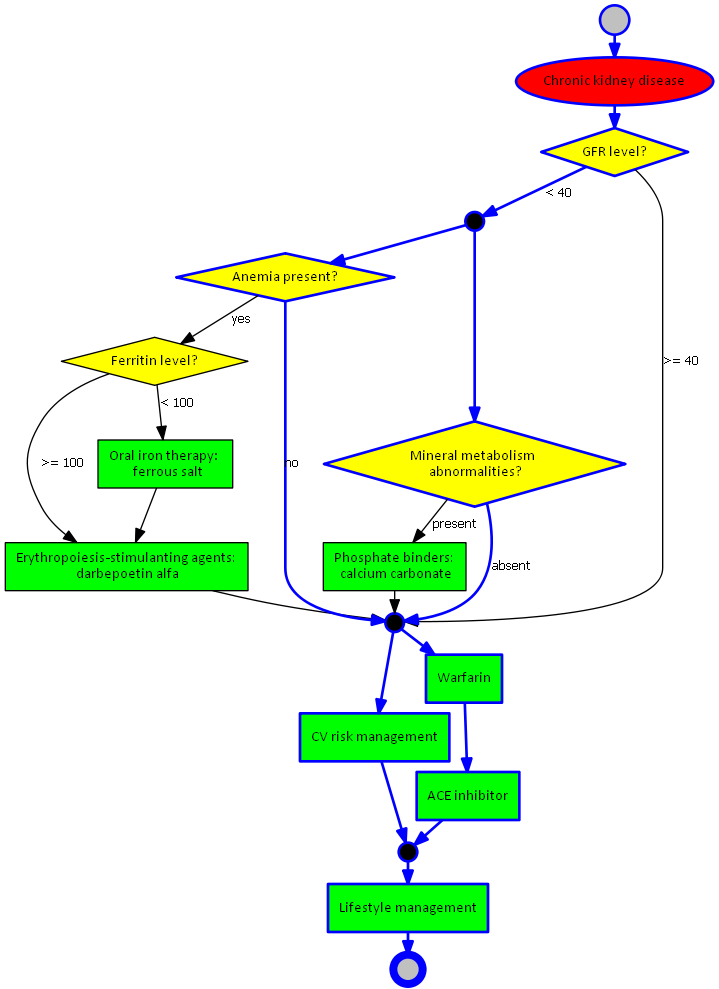
\includegraphics[scale=0.4]{img/rozwiazanie1ckd-simplified-ver-5_przyklad.png}
\caption{Wytyczne dla przewlekłej choroby nerek}
\label{fig:ckd_rozw}
\end{figure}